\documentclass[../main.tex]{subfiles}
%!TEX root = ./appendixNylonShaftScrew.tex
\graphicspath {{../}}

\begin{document}
\section{Vectoring Shaft Screw Axial Loading Conditions} \label{axialShaft}
The screw which secures the nylon vectoring shaft is part of the servo motor assembly. The servo motor output is a spline with a female thread for a 3mm screw to be threaded into (Servo example from ServoCity \cite{SPLINE}), as shown in Figure \ref{fig:servoSpline}.

\begin{figure}[H]
	\centering
	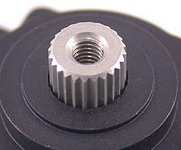
\includegraphics[width=.5\linewidth]{img/servo/spline.PNG}
	\caption{HS-7950TH Servo Spline Attachment \cite{SPLINE}}
	\label{fig:servoSpline}
\end{figure}

One potential concern would be for the small 3mm screw (which threads into the spline) breaking if an axial load was applied to it. While there is \textit{theoretically} no scenario where any axial load is applied, it is worth checking the strength of the screw, because during transportation of the airship it is possible that the part may be unintentionally pulled. To find the proof force of the bolt, it was assumed that the bolt was a SAE Class 4.8 M3-0.5, and the following properties were found:

\begin{table}[H]
	\centering
	\caption{Table of Bolt Strength for a M3-0.5 Bolt \cite{BOLTSTRENGTH}}
	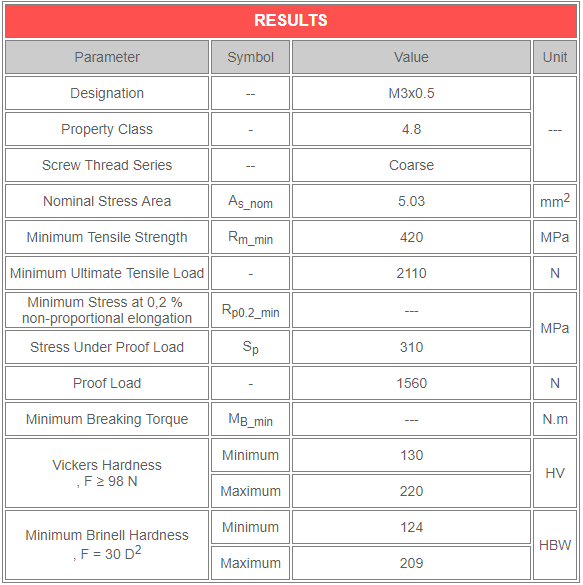
\includegraphics[width=\linewidth]{img/servo/boltProperties.PNG}
	\label{tbl:boltStrength}
\end{table}

Based on this, the tensile load of the bolt is 2110N, which is much higher than any axial forces that the shaft is expected to have to withstand. Therefore the design is not a problem.

\end{document}